\chapter{Entropie des trous noirs, holographie et espace de de Sitter}

\lectureoverview{Nous achevons l’argument de correspondance amorcé au cours précédent. L’entropie d’une corde très excitée est proportionnelle à sa masse, tandis que celle d’un trou noir de Schwarzschild est proportionnelle à son aire. Ces deux formules ne se relient pas en identifiant un trou noir fortement gravitant à une corde libre, mais en faisant varier lentement le couplage des cordes jusqu’à ce que les deux descriptions se rejoignent. La loi en aire mène alors naturellement au principe holographique, et la dernière partie du cours introduit l’espace en expansion et la géométrie de de Sitter, dont nous étudierons l’horizon au prochain cours.}

\section{Retour au problème de dénombrement}

Il restait un point à régler dans le dénombrement des cordes longues. Si l’on répartit une longueur totale fixe entre plusieurs cordes, des cordes identiques de même longueur sont indiscernables. Leurs positions dans la boîte font néanmoins partie de l’état, et la boîte est choisie de façon à avoir à peu près la taille de la région occupée par la corde longue correspondante.

\begin{classroomqa}
\audiencequestion{Les cordes courtes sont-elles distinguables les unes des autres, et leurs positions comptent-elles ?\lecturetimestamp{00:00:37}}
\lecturerresponse{Des cordes aux propriétés identiques sont indiscernables, mais on dénombre leurs positions dans la boîte. La comparaison se fait à volume fixé, choisi pour correspondre à la région occupée par la corde longue.}
\end{classroomqa}

Cela réglé, nous pouvons énoncer l’objectif. Nous allons rassembler une courte liste d’équations et nous en servir pour obtenir la dépendance de l’entropie d’un trou noir. Aucun intégrale ni aucune somme infinie n’est nécessaire. La difficulté n’est pas algébrique : elle consiste à savoir quelles grandeurs peuvent être comparées et à quel stade du raisonnement.

\section{Unités naturelles et aire de Planck}

Posons
\begin{equation}
c=\hbar=1,
\label{eq:l07-natural-units}
\end{equation}
mais gardons explicite la constante de Newton. Il en découle d’abord que le temps et la longueur ont les mêmes unités. La relation pour les photons
\begin{equation}
E=\frac{\hbar c}{\lambda}
\end{equation}
et la relation masse-énergie \(E=mc^2\) impliquent alors
\begin{equation}
[M]=L^{-1}.
\label{eq:l07-mass-dimension}
\end{equation}
On peut donc exprimer une masse en inverse d’une longueur.

\begin{figure}[htbp]
\centering
\includegraphics[width=0.62\textwidth]{lecture_07_figure_02.png}
\caption{Convention des unités naturelles au début de l’argument dimensionnel. La formule de l’énergie est complétée par les équations ci-dessus.}
\lectureframe{00:03:27.900}
\end{figure}

Pour déterminer les unités de \(G_N\), utilisons l’accélération newtonienne à seule fin de tenir compte des dimensions :
\begin{equation}
a\sim\frac{G_NM}{R^2}.
\end{equation}
Comme \(T\) et \(L\) ont les mêmes unités, \([a]=L/T^2=L^{-1}\). Avec l’équation~\eqref{eq:l07-mass-dimension}, cela donne
\begin{equation}
[G_N]=L^2.
\end{equation}
Dans ces unités, la constante de Newton a les dimensions d’une aire. En définissant la longueur de Planck par
\begin{equation}
G_N=\ell_p^2,
\label{eq:l07-planck-area}
\end{equation}
on comprend aussitôt pourquoi \(A/G_N=A/\ell_p^2\) est sans dimension : elle mesure une aire en unités d’aire de Planck.

\section{Le couplage des cordes et l’intensité de la gravitation}

Il faut maintenant traduire la gravitation dans le langage des cordes. L’image utile est celle d’un processus d’échange. Lorsqu’une corde se croise elle-même, elle peut se scinder puis se rejoindre. Une petite boucle de corde fermée peut être émise par un objet et absorbée par un autre ; si cette excitation est un graviton, le processus véhicule la gravitation. Un facteur d’interaction intervient à l’émission, un autre à l’absorption : l’intensité de l’échange comporte donc \(g_s^2\).

Le couplage \(g_s\) est sans dimension. Plus précisément, c’est un couplage au niveau des amplitudes, tandis qu’une probabilité ou un taux apparaît à l’ordre \(g_s^2\).\editorialnote{Dans le cours, \(g_s\) est parfois appelé une probabilité, puis le propos est rectifié : il s’agit de la racine carrée d’une probabilité. Le couplage perturbatif intervient au niveau des amplitudes.} Comme \(G_N\) a les dimensions d’une aire, il manque encore une échelle de longueur. La longueur fondamentale des cordes \(\ell_s\), qui caractérise une oscillation élémentaire de corde, la fournit :
\begin{equation}
G_N\sim g_s^2\ell_s^2,
\qquad
\ell_p\sim g_s\ell_s.
\label{eq:l07-planck-string}
\end{equation}

\begin{figure}[htbp]
\centering
\includegraphics[width=0.72\textwidth]{lecture_07_figure_05.png}
\caption{Relation entre les couplages inscrite au tableau : \(G_N=\ell_p^2\) et \(g_s^2\ell_s^2\sim\ell_p^2\).}
\lectureframe{00:12:15.000}
\end{figure}

À faible couplage, \(g_s\ll1\), la longueur de Planck est très inférieure à la longueur des cordes. Diminuer \(g_s\) affaiblit la gravitation tout en laissant fixe l’échelle de longueur élémentaire des cordes.\editorialnote{Dans une théorie effective à quatre dimensions, les données de compactification et les conventions numériques interviennent également dans \(G_N\). Elles sont maintenues fixes et omises dans cet argument d’échelle.}

\section{Dénombrement d’une corde longue}

L’entropie dénombre les choix élémentaires nécessaires pour spécifier un état. Représentons une corde très excitée par une marche sur un réseau carré. À chaque sommet, le lien suivant peut pointer dans l’une de quatre directions. Décrire le choix élémentaire comme une décision à quatre possibilités ou comme deux décisions binaires ne change qu’une constante d’ordre unité. Ce qui importe, c’est le nombre de pas.

Si \(L\) est la longueur de contour de la corde et si chaque pas a pour longueur \(\ell_s\), il faut
\begin{equation}
N=\frac{L}{\ell_s}
\end{equation}
pas. Le nombre de marches croît exponentiellement, schématiquement comme \(\Omega_N\sim q^N\), où \(q\) est d’ordre unité ; on obtient donc
\begin{equation}
S_{\mathrm{str}}=\log\Omega_N\sim N\sim\frac{L}{\ell_s}.
\label{eq:l07-string-entropy-length}
\end{equation}

\begin{figure}[htbp]
\centering
\includegraphics[width=0.68\textwidth]{lecture_07_figure_03.png}

\vspace{0.7em}
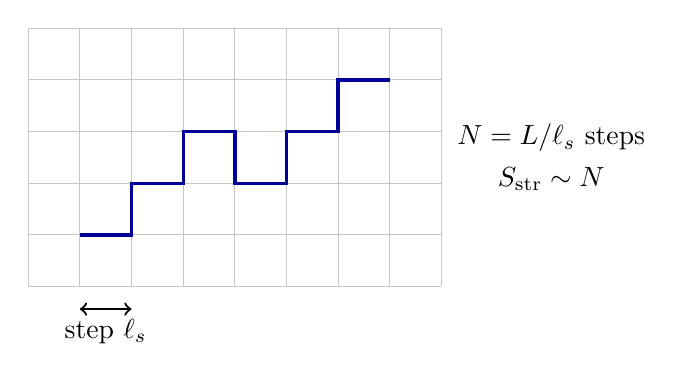
\begin{tikzpicture}[scale=0.82]
  \draw[step=0.8cm,gray!45,thin] (0,0) grid (6.4,4.0);
  \draw[very thick,blue!60!black]
    (0.8,0.8)--(1.6,0.8)--(1.6,1.6)--(2.4,1.6)--(2.4,2.4)--
    (3.2,2.4)--(3.2,1.6)--(4.0,1.6)--(4.0,2.4)--(4.8,2.4)--
    (4.8,3.2)--(5.6,3.2);
  \draw[<->,thick] (0.8,-0.35)--(1.6,-0.35);
  \node[below] at (1.2,-0.35) {step \(\ell_s\)};
  \node[align=center] at (8.1,2.0) {\(N=L/\ell_s\) steps\\[0.3em]\(S_{\mathrm{str}}\sim N\)};
\end{tikzpicture}
\caption{Modèle sur réseau inscrit au tableau et interprétation épurée en termes de marche aléatoire. C’est la longueur de contour, et non le diamètre de la boule emmêlée, qui détermine le nombre de choix.}
\lectureframe{00:17:20.000}
\end{figure}

On dénombre la masse à partir des mêmes segments élémentaires. Un segment de longueur \(\ell_s\) a une échelle de masse de
\begin{equation}
m_{\mathrm{seg}}\sim\frac{1}{\ell_s}.
\end{equation}

\begin{classroomqa}
\audiencequestion{Attribue-t-on au segment élémentaire la longueur \(\ell_s\) ?\lecturetimestamp{00:18:56}}
\lecturerresponse{Oui. Sa longueur caractéristique est \(\ell_s\), donc, en unités naturelles, sa masse caractéristique est \(1/\ell_s\).}
\end{classroomqa}

En additionnant les masses des segments \(L/\ell_s\), on obtient
\begin{equation}
M\sim\frac{L}{\ell_s}\frac{1}{\ell_s}
=\frac{L}{\ell_s^2},
\qquad
L\sim M\ell_s^2.
\label{eq:l07-string-mass}
\end{equation}
Cette relation d’échelle condense les énergies cinétique et potentielle de la corde oscillante ; un traitement détaillé de mécanique statistique donne la même dépendance. En substituant dans l’équation~\eqref{eq:l07-string-entropy-length}, on obtient la formule pour la corde dont nous aurons besoin :
\begin{equation}
S_{\mathrm{str}}\sim M\ell_s.
\label{eq:l07-string-entropy-mass}
\end{equation}

\begin{figure}[htbp]
\centering
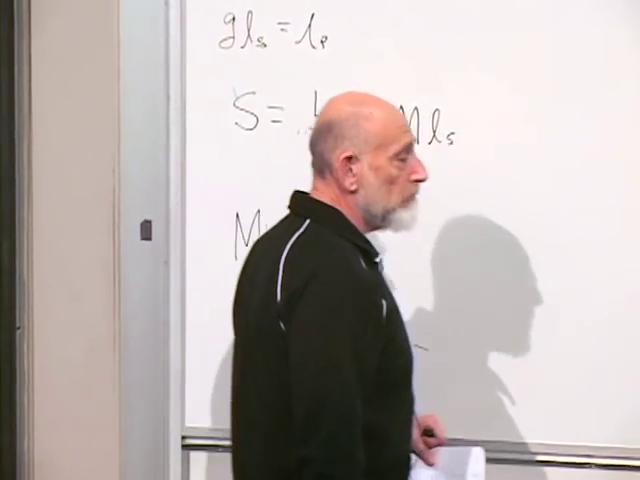
\includegraphics[width=0.66\textwidth]{lecture_07_figure_04.png}
\caption{La colonne consacrée aux cordes, assemblée avant la comparaison : \(\ell_p\sim g_s\ell_s\), \(S_{\mathrm{str}}\sim L/\ell_s\sim M\ell_s\) et \(M\sim L/\ell_s^2\).}
\lectureframe{00:21:57.800}
\end{figure}

\section{Pourquoi une corde libre n’est pas encore un trou noir}

Du côté gravitationnel, la formule semi-classique exacte est
\begin{equation}
S_{\mathrm{BH}}=\frac{A}{4G_N}.
\label{eq:l07-bh-exact}
\end{equation}

\begin{classroomqa}
\audiencequestion{Quel coefficient numérique faut-il mettre au dénominateur ?\lecturetimestamp{00:23:28}}
\lecturerresponse{Quatre. L’argument de correspondance retrouvera la dépendance d’échelle, mais il est trop grossier pour déterminer ce facteur exact.}
\end{classroomqa}

Pour un trou noir de Schwarzschild à quatre dimensions,
\begin{equation}
R_s=2G_NM,
\qquad
A=4\pi R_s^2.
\end{equation}
En négligeant les constantes numériques comme dans le cours,
\begin{align}
S_{\mathrm{BH}}
&\sim\frac{A}{G_N}
\sim\frac{(G_NM)^2}{G_N} \\
&\sim M^2G_N
\sim M^2\ell_p^2.
\label{eq:l07-bh-scaling}
\end{align}

\begin{figure}[htbp]
\centering
\includegraphics[width=0.72\textwidth]{lecture_07_figure_06.png}
\caption{Comparaison achevée au tableau : l’entropie de la corde est une longueur exprimée en unités de corde, tandis que celle du trou noir est une aire exprimée en unités de Planck.}
\lectureframe{00:25:35.000}
\end{figure}

La ressemblance entre les équations~\eqref{eq:l07-string-entropy-mass} et \eqref{eq:l07-bh-scaling} est suggestive, mais ce ne sont pas les mêmes formules. Il serait erroné de simplement qualifier de corde libre le trou noir initial et de faire la substitution. Le dénombrement d’une corde libre omet l’interaction attractive entre ses différentes parties, précisément celle qui compacte la corde en trou noir et abaisse son énergie totale par une énergie de liaison négative.

L’exemple d’une étoile rend l’erreur familière. Un gaz chaud de masse stellaire placé dans une boîte trop grande ne constitue pas un modèle d’étoile, même à la même température. L’auto-gravitation modifie la taille d’équilibre et la relation entre énergie et entropie. Suivre chacune des auto-interactions d’une corde longue serait difficile ; nous allons donc éviter de le faire.

\begin{classroomqa}
\audiencequestion{Si une petite boucle quitte une corde longue, son entropie diminue. L’échange de gravitons réduit-il donc l’entropie du système gravitant ?\lecturetimestamp{00:28:48}}
\lecturerresponse{Pas dans le processus d’échange à l’équilibre considéré ici. Des excitations virtuelles sont émises et absorbées dans les deux sens ; le schéma ne représente pas la perte littérale d’un fragment permanent de corde. Il sert uniquement, pour l’instant, à établir les deux facteurs de couplage et donc la dépendance en \(g_s^2\).}
\end{classroomqa}

\section{Le jeu de correspondance adiabatique}

Partons plutôt d’un régime où la gravitation est négligeable. Lorsque \(g_s\to0\), les cordes se croisent sans se scinder ni se rejoindre, et l’attraction gravitationnelle propre disparaît. Augmentons \(g_s\) en gardant \(\ell_s\) fixe : la gravitation se renforce, une corde très excitée se contracte et finit par devenir un trou noir. Si l’on inverse lentement le réglage, le trou noir doit redevenir un état de corde. Il peut se transformer en un petit nombre de cordes longues, mais le dénombrement à haute énergie du cours précédent indique que le secteur dominant contient une corde longue plutôt qu’un gaz immense de cordes courtes.

\begin{classroomqa}
\audiencequestion{Que maintient-on fixe pendant la variation du couplage ?\lecturetimestamp{00:32:19}}
\lecturerresponse{La longueur des cordes \(\ell_s\), et donc l’échelle de masse élémentaire des cordes \(1/\ell_s\), restent fixes. Le réglage modifie \(g_s\) et, par conséquent, \(G_N\sim g_s^2\ell_s^2\).}
\end{classroomqa}

La variation doit être lente, isolée et réversible. Dans ces conditions, l’entropie est un invariant adiabatique :
\begin{equation}
\Delta S=0.
\label{eq:l07-adiabatic}
\end{equation}
La lenteur ne suffit pas si des transitions dissipatives ou incontrôlées se produisent. Ici, ``adiabatique'' signifie que l’on peut suivre continûment une même famille d’états.\editorialnote{C’est le sens thermodynamique réversible du terme adiabatique. Un processus irréversible peut être adiabatique au sens d’une absence d’échange de chaleur et tout de même produire de l’entropie.}

Soit un trou noir cible de masse \(M_0\) et de couplage \(g_{s,0}\). Avant d’utiliser la formule de l’aire que nous cherchons à expliquer, l’analyse dimensionnelle indique seulement que l’entropie d’un trou noir neutre et non rotatif est une fonction de la combinaison sans dimension
\begin{equation}
S_{\mathrm{BH}}=f(M\ell_p)
=f(Mg_s\ell_s).
\label{eq:l07-entropy-function}
\end{equation}
À \(\ell_s\) fixé, un chemin isentropique conserve donc
\begin{equation}
Mg_s=M_0g_{s,0}
\label{eq:l07-adiabat}
\end{equation}
à condition de suivre la même branche d’états.

Quand \(g_s\) diminue, l’énergie de liaison négative est éliminée ; la masse \(M\) augmente donc le long de ce chemin. La configuration de corde sous-jacente est également moins fortement liée et s’étend. En revanche, le rayon de Schwarzschild formel évolue comme \(R_s\sim Mg_s^2\ell_s^2\sim g_s\ell_s\) sur l’adiabatique et diminue donc.\editorialnote{Dans la discussion orale, le terme ``grandit'' désigne l’objet libéré de sa liaison gravitationnelle. Il ne faut pas l’interpréter comme une augmentation du rayon de Schwarzschild le long de l’adiabatique déduite ici.}

\begin{classroomqa}
\audiencequestion{L’objet grandit-il ou rétrécit-il lorsque la gravitation s’affaiblit ?\lecturetimestamp{00:36:28}}
\lecturerresponse{Sa structure de corde est libérée et s’étend, tandis que sa masse augmente parce que l’énergie de liaison négative est éliminée. Le rayon attribué par la formule du trou noir diminue jusqu’à atteindre l’échelle des cordes, où cette description en trou noir cesse d’être utile.}
\end{classroomqa}

\section{Deux courbes et leur intersection}

Plaçons la masse en ordonnée et le couplage des cordes en abscisse. L’équation~\eqref{eq:l07-adiabat} est une hyperbole, \(M\propto g_s^{-1}\).

\begin{classroomqa}
\audiencequestion{Quel type de courbe correspond à un produit constant \(Mg_s\) ?\lecturetimestamp{00:44:08}}
\lecturerresponse{Une hyperbole. C’est l’adiabatique passant par le point cible \((g_{s,0},M_0)\).}
\end{classroomqa}

La seconde courbe marque le passage d’une description à l’autre. Un trou noir ne peut plus être décrit par une géométrie de Schwarzschild classique lorsque son rayon est inférieur à celui d’une oscillation élémentaire de corde. Nous estimons donc le point de correspondance par
\begin{equation}
R_s\sim\ell_s.
\label{eq:l07-correspondence-radius}
\end{equation}
En utilisant \(R_s\sim MG_N\) et l’équation~\eqref{eq:l07-planck-string}, on obtient
\begin{equation}
Mg_s^2\ell_s^2\sim\ell_s,
\qquad
Mg_s^2\sim\frac{1}{\ell_s}.
\label{eq:l07-transition-curve}
\end{equation}
La courbe de transition décroît donc comme \(M\propto g_s^{-2}\), plus rapidement que l’adiabatique.

\begin{figure}[htbp]
\centering
\includegraphics[width=0.70\textwidth]{lecture_07_figure_07.png}

\vspace{0.6em}
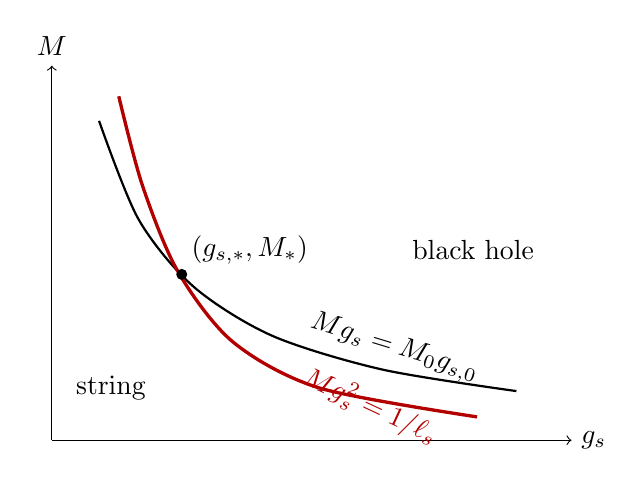
\begin{tikzpicture}[x=1cm,y=0.78cm]
  \draw[->] (0.4,0.4)--(7.0,0.4) node[right] {\(g_s\)};
  \draw[->] (0.4,0.4)--(0.4,6.5) node[above] {\(M\)};
  \draw[thick,black] plot[smooth] coordinates {(1.0,5.6) (1.5,4.0) (2.2,2.9) (3.2,2.1) (4.6,1.55) (6.3,1.2)};
  \draw[very thick,red!70!black] plot[smooth] coordinates {(1.25,6.0) (1.55,4.55) (2.0,3.15) (2.7,2.0) (3.8,1.25) (5.8,0.78)};
  \fill (2.05,3.1) circle (2pt) node[above right] {\((g_{s,*},M_*)\)};
  \node[black,rotate=-17] at (4.75,1.9) {\(Mg_s=M_0g_{s,0}\)};
  \node[red!70!black,rotate=-25] at (4.45,0.95) {\(Mg_s^2=1/\ell_s\)};
  \node at (5.75,3.5) {black hole};
  \node at (1.15,1.25) {string};
\end{tikzpicture}
\caption{Graphique du tableau et interprétation épurée. L’adiabatique noire coupe la courbe de correspondance rouge, plus pentue, au point où l’objet devient semblable à une corde.}
\lectureframe{00:49:35.000}
\end{figure}

À l’intersection \((M_*,g_{s,*})\), les deux équations sont
\begin{align}
M_*g_{s,*} &= M_0g_{s,0}, \\
M_*g_{s,*}^2 &\sim \frac{1}{\ell_s}.
\end{align}
Élevons la première équation au carré et divisons par la seconde :
\begin{equation}
M_*
\sim M_0^2g_{s,0}^2\ell_s.
\end{equation}
En multipliant par \(\ell_s\),
\begin{equation}
M_*\ell_s
\sim M_0^2g_{s,0}^2\ell_s^2
\sim M_0^2G_{N,0}.
\label{eq:l07-crossover-result}
\end{equation}

\begin{figure}[htbp]
\centering
\includegraphics[width=0.68\textwidth]{lecture_07_figure_08.png}
\caption{Calcul achevé du passage d’un régime à l’autre, y compris \(M_*\ell_s=M_0^2g_{s,0}^2\ell_s^2=M_0^2G_{N,0}\).}
\lectureframe{00:54:40.000}
\end{figure}

\begin{classroomqa}
\audiencequestion{En divisant les équations des deux courbes, \(\ell_s\) se retrouve-t-il au numérateur ou au dénominateur ?\lecturetimestamp{00:52:41}}
\lecturerresponse{Au numérateur. Diviser par \(1/\ell_s\) revient à multiplier par \(\ell_s\), d’où \(M_*\sim M_0^2g_{s,0}^2\ell_s\).}
\end{classroomqa}

Au point de transition, la formule pour la corde est valable, donc
\begin{equation}
S_*\sim M_*\ell_s.
\end{equation}
L’entropie est restée inchangée le long du chemin. En combinant ce résultat avec l’équation~\eqref{eq:l07-crossover-result}, on obtient l’entropie du trou noir cible initial :
\begin{equation}
S_{\mathrm{BH}}(M_0)
\sim M_0^2G_{N,0}
\sim M_0^2\ell_{p,0}^2.
\label{eq:l07-final-correspondence}
\end{equation}
C’est la dépendance en aire recherchée.

\section{Ce que la correspondance démontre et ne démontre pas}

Cette construction n’affirme pas que le trou noir initial, fortement gravitant, est une corde libre. Elle amène l’objet dans un régime où le dénombrement des cordes est fiable, en déduit l’entropie, puis reporte cette entropie le long d’un chemin réversible. La transition est un passage continu plutôt qu’une frontière de phase située précisément ; cette estimation ne peut donc déterminer le coefficient \(1/4\) de l’équation~\eqref{eq:l07-bh-exact}.

Le même raisonnement fonctionne néanmoins, à un facteur près, pour les trous noirs chargés, les objets noirs dans d’autres dimensions et les branes noires étendues. Des exemples plus symétriques et supersymétriques permettent des dénombrements protégés d’états, qui conservent une information exacte lorsque le couplage varie ; ces méthodes retrouvent les coefficients numériques, mais exigent un appareil mathématique dont l’argument conceptuel présenté ici n’a pas besoin.

Surtout, le calcul fournit une interprétation microscopique. L’entropie témoigne d’une structure cachée. La mécanique des fluides décrit la densité, la pression et l’écoulement sans faire intervenir les molécules ; l’entropie du fluide révèle l’existence de ces degrés de liberté microscopiques. De même, la relativité générale décrit un horizon sans montrer ses microétats. Le dénombrement des cordes montre qu’une théorie quantique cohérente de la gravitation peut contenir assez d’états pour rendre compte de l’entropie du trou noir.

\begin{classroomqa}
\audiencequestion{Qu’aurait donné \(S\sim M^3\ell_p^3\) à la place du résultat quadratique ?\lecturetimestamp{00:59:41}}
\lecturerresponse{On aurait obtenu une loi en volume. L’entropie de la matière ordinaire dans une pièce ou d’une tasse de café est proportionnelle au volume ; le résultat quadratique est particulier parce que, par l’intermédiaire de \(R_s\sim M\ell_p^2\), il est proportionnel à l’aire de l’horizon.}
\end{classroomqa}

Le résultat indique que l’entropie de Bekenstein--Hawking n’est pas une simple analogie thermodynamique formelle. Elle signale l’existence de degrés de liberté gravitationnels microscopiques, même si la dérivation élémentaire ne permet pas de les voir un à un.

\section{De l’entropie maximale à l’holographie}

Changeons maintenant de question. Au lieu de demander quelle est l’entropie d’un état donné, cherchons l’entropie maximale compatible avec une région.

Partons d’un modèle ordinaire de pièce sur réseau. Découpons le volume en cellules de taille \(V_{\mathrm{cell}}\), et attribuons à chacune une question binaire : occupée ou vide. Susskind donne à l’atome imaginaire le nom délibérément absurde de ``meatonium'', afin que les détails réalistes de la structure atomique ne détournent pas l’attention du dénombrement. Si
\begin{equation}
N=\frac{V}{V_{\mathrm{cell}}},
\end{equation}
alors le nombre de configurations et l’entropie maximale sont
\begin{equation}
\Omega=2^N,
\qquad
S_{\max}=\log\Omega=N\log2
\sim\frac{V}{V_{\mathrm{cell}}}.
\label{eq:l07-volume-count}
\end{equation}

\begin{figure}[htbp]
\centering
\includegraphics[width=0.68\textwidth]{lecture_07_figure_09.png}
\caption{La pièce découpée en cellules, chacune dans l’un de deux états. On dénombre une entropie maximale, et non l’entropie de la pièce bien rangée où se trouve la classe.}
\lectureframe{01:05:20.000}
\end{figure}

La pièce réelle est très loin de ce maximum. Un état explorant de manière chaotique tous ces choix dans les cellules serait extrêmement chaud. Ce que l’on retient du modèle jouet, c’est l’attente habituelle : le nombre de degrés de liberté indépendants, et donc l’entropie maximale, varie comme le volume.

La gravitation bouleverse cette attente. Considérons une région sphérique de frontière d’aire \(A\), d’entropie initiale \(S_{\mathrm{i}}\) et de masse \(M\), inférieure à la masse \(M_{\mathrm{BH}}\) du trou noir qui remplirait tout juste la sphère. Si \(M\) était plus grande, son horizon s’étendrait déjà au-delà de la frontière choisie.

Faisons maintenant entrer une coquille de masse \(M_{\mathrm{BH}}-M\). Sa composition n’a pas d’importance ; le cours envisage de la lumière, de la matière ordinaire ou même du fromage suisse. Organisons son effondrement. L’état final est un trou noir dont l’horizon remplit tout juste la région et dont l’entropie vaut
\begin{equation}
S_{\mathrm{f}}=\frac{A}{4G_N}.
\end{equation}
La deuxième loi impose
\begin{equation}
S_{\mathrm{i}}\le S_{\mathrm{f}}
=\frac{A}{4G_N}.
\label{eq:l07-holographic-bound}
\end{equation}

\begin{figure}[htbp]
\centering
\includegraphics[width=0.70\textwidth]{lecture_07_figure_10.png}

\vspace{0.5em}
\begin{tikzpicture}[scale=0.88]
  \draw[thick] (0,0) circle (1.35);
  \draw[very thick,red!70!black] (0,0) circle (2.05);
  \fill[gray!25] (0,0) circle (1.32);
  \node at (0,0) {\(M,S_{\mathrm{i}}\)};
  \draw[-{Latex[length=3mm]},thick,red!70!black] (3.5,0)--(2.15,0);
  \node[align=center,right] at (3.5,0) {incoming shell\\\(M_{\mathrm{BH}}-M\)};
  \node[below] at (0,-2.2) {final horizon area \(A\)};
\end{tikzpicture}
\caption{Construction avec une coquille. On fait entrer suffisamment de masse supplémentaire pour former un trou noir dont l’horizon remplit tout juste la région choisie.}
\lectureframe{01:13:30.000}
\end{figure}

Comme un trou noir de cette taille est un état admissible et qu’il sature l’inégalité, l’entropie maximale est
\begin{equation}
S_{\max}=\frac{A}{4G_N}.
\label{eq:l07-holographic-maximum}
\end{equation}
C’est le principe holographique sous forme de dénombrement : le nombre maximal de degrés de liberté indépendants dans une région gravitationnelle varie comme l’aire de sa frontière, soit approximativement un degré de liberté d’ordre unité par aire de Planck, plutôt que comme le nombre de volumes de Planck qu’elle contient.\editorialnote{L’argument de la coquille suppose que l’on peut enfermer la région et provoquer son effondrement de la manière décrite. Les espaces-temps plus généraux exigent des bornes covariantes sur l’entropie, mais l’argument sphérique saisit le principe utilisé dans le cours.}

L’écart est immense. L’intuition issue de la théorie locale des champs suggère que les choix effectués en différents points intérieurs devraient se combiner indépendamment et produire une loi en volume. La gravitation indique qu’un nombre suffisant de tels choix provoquerait l’effondrement de la région, et le trou noir fournit l’entropie admissible maximale. Le dénombrement par la frontière n’est donc pas une petite correction au dénombrement volumique : l’espace de Hilbert est organisé d’une manière différente.

\begin{classroomqa}
\audiencequestion{Que se passe-t-il dans un univers très vaste de densité à peu près uniforme ?\lecturetimestamp{01:15:48}}
\lecturerresponse{Cette question relève de la cosmologie plutôt que de la construction sphérique statique. Elle nous conduit à examiner les solutions en expansion des équations d’Einstein.}
\end{classroomqa}

\begin{classroomqa}
\audiencequestion{La borne en aire est-elle liée au principe d’incertitude ?\lecturetimestamp{01:16:03}}
\lecturerresponse{Le cours laisse cette question ouverte et passe ensuite à la cosmologie.}
\end{classroomqa}

\section{L’espace en expansion}

Nous ne dériverons pas ici les solutions cosmologiques à partir des équations d’Einstein ; nous les écrirons et apprendrons à les lire. Les tranches spatiales peuvent être fermées et à courbure positive, hyperboliques et à courbure négative, ou plates. Pour la discussion présente, considérons des tranches euclidiennes plates dans un espace-temps dépendant du temps.

\begin{classroomqa}
\audiencequestion{Quel est l’analogue de l’espace euclidien ordinaire pour l’espace-temps ?\lecturetimestamp{01:19:37}}
\lecturerresponse{L’espace de Minkowski. La cosmologie étudiée ici possède des tranches spatiales plates, mais son espace-temps n’est pas celui de Minkowski, car la métrique spatiale varie avec le temps.}
\end{classroomqa}

L’image familière du ballon décrit une surface fermée en expansion dans une dimension de moins. Susskind se souvient d’avoir tenté la démonstration avec un grand ballon marqué ; le marqueur a fragilisé le caoutchouc et provoqué un véritable éclatement. Cet incident met aussi en évidence un défaut conceptuel de l’analogie. Quand un ballon ordinaire se dilate, ses molécules de caoutchouc s’écartent et le matériau s’amincit jusqu’à se rompre. L’espace cosmologique ne voit pas ses lois locales se diluer. Pour préserver l’analogie, il faut imaginer que l’on ajoute sans cesse de nouvelles molécules de caoutchouc, afin que chaque petite région conserve les mêmes propriétés locales. Dans un modèle plat, remplaçons le ballon par une grande feuille que l’on étire uniformément et que l’on renouvelle de la même façon.

Mathématiquement, l’expansion figure dans la métrique :
\begin{equation}
\begin{aligned}
ds^2&=-dt^2+a(t)^2d\mathbf{x}^2,\\
d\mathbf{x}^2&=\delta_{ij}\,dx^i dx^j
=dx^2+dy^2+dz^2.
\end{aligned}
\label{eq:l07-frw-metric}
\end{equation}

\begin{figure}[htbp]
\centering
\includegraphics[width=0.72\textwidth]{lecture_07_figure_11.png}
\caption{Métrique d’expansion spatialement plate telle qu’elle est inscrite au tableau.}
\lectureframe{01:25:10.000}
\end{figure}

On appelle comobiles les points dont les coordonnées spatiales restent fixes. Si deux points comobiles ont une séparation coordonnée \(\Delta x\), leur distance propre à l’instant \(t\) vaut
\begin{equation}
D(t)=a(t)\Delta x.
\label{eq:l07-proper-distance}
\end{equation}
Leurs coordonnées ne varient pas, mais la distance métrique qui les sépare change. En dérivant à \(\Delta x\) fixe,
\begin{equation}
V=\dot D=\dot a\,\Delta x
=\frac{\dot a}{a}D.
\end{equation}
Définissons le paramètre de Hubble
\begin{equation}
H(t)=\frac{\dot a(t)}{a(t)}.
\label{eq:l07-hubble-parameter}
\end{equation}
Alors
\begin{equation}
V=H(t)D,
\label{eq:l07-hubble-law}
\end{equation}
C’est la loi de Hubble à un instant cosmique donné.

\begin{figure}[htbp]
\centering
\includegraphics[width=0.68\textwidth]{lecture_07_figure_12.png}
\caption{Loi de récession à temps égal inscrite au tableau : \(V=D\,\dot a/a\).}
\lectureframe{01:29:10.000}
\end{figure}

Le nom ``constante de Hubble'' peut induire en erreur. En général, \(H(t)\) varie avec le temps. Ce qui est constant dans l’espace, c’est le rapport \(V/D\) pour toute paire de points comobiles sur une même tranche de temps.

\begin{classroomqa}
\audiencequestion{Pour les galaxies lointaines, à quelle époque correspond le temps dans cette relation ? Nous les observons à une époque antérieure.\lecturetimestamp{01:31:10}}
\lecturerresponse{L’équation~\eqref{eq:l07-hubble-law} est une relation à temps égal. Une observation suit un rayon lumineux dirigé vers le passé et capte donc la galaxie lointaine à un instant antérieur ; la relation entre le décalage vers le rouge mesuré et la distance dépend donc de toute l’histoire le long du cône de lumière, et non d’une valeur instantanée de \(H\).}
\end{classroomqa}

\begin{figure}[htbp]
\centering
\includegraphics[width=0.66\textwidth]{lecture_07_figure_13.png}
\caption{Schéma d’espace-temps servant à distinguer une séparation à temps égal de ce qu’un observateur voit le long d’un rayon lumineux dirigé vers le passé.}
\lectureframe{01:33:20.000}
\end{figure}

\section{L’échelle de Hubble et l’expansion de de Sitter}

En unités \(c=1\), l’équation~\eqref{eq:l07-hubble-law} associe une vitesse de récession égale à 1 à la distance
\begin{equation}
D_H=\frac{1}{H}.
\label{eq:l07-hubble-radius}
\end{equation}
Des points comobiles plus éloignés peuvent avoir \(V>1\), voire \(V\gg1\), sans violer la relativité restreinte. Ils ne dépassent pas la vitesse de la lumière par rapport à un observateur local ; leur distance propre augmente parce que la géométrie intermédiaire se dilate.\editorialnote{Dans une cosmologie générale dépendant du temps, \(1/H\) est le rayon de Hubble, qui n’est pas automatiquement un horizon des événements. Dans le cas de de Sitter étudié ensuite, il devient l’échelle d’horizon constante.}

Dans de nombreux anciens modèles cosmologiques en décélération, \(H(t)\) diminue et \(1/H(t)\) augmente, si bien que des régions autrefois en récession supraluminique peuvent ensuite entrer en contact causal. Le tableau de l’avenir lointain décrit dans le cours tend plutôt vers une valeur positive constante \(H\). Alors \(1/H\) reste fixe, et l’équation d’expansion devient
\begin{equation}
\frac{\dot a}{a}=H,
\qquad
\dot a=Ha.
\label{eq:l07-constant-h}
\end{equation}

\begin{classroomqa}
\audiencequestion{Quelles sont les unités d’un paramètre de Hubble constant ?\lecturetimestamp{01:38:24}}
\lecturerresponse{L’inverse d’un temps. De manière équivalente, avec \(c=1\), c’est l’inverse d’une longueur. La grandeur \(H^{-1}\) fournit à la fois une échelle de temps d’expansion et une échelle de distance ; le cours donne comme exemple un ordre de grandeur d’environ quinze milliards d’années.}
\end{classroomqa}

La solution de l’équation~\eqref{eq:l07-constant-h} est
\begin{equation}
a(t)=a_0e^{Ht}.
\label{eq:l07-desitter-scale-factor}
\end{equation}

\begin{classroomqa}
\audiencequestion{Quelle fonction a un taux de variation proportionnel à elle-même ?\lecturetimestamp{01:39:04}}
\lecturerresponse{Une exponentielle. Le facteur d’échelle est donc \(a_0e^{Ht}\), tandis que le coefficient spatial \(a(t)^2\) de la métrique croît comme \(e^{2Ht}\).}
\end{classroomqa}

\begin{figure}[htbp]
\centering
\includegraphics[width=0.70\textwidth]{lecture_07_figure_14.png}
\caption{Équations à \(H\) constant et leur solution exponentielle inscrites au tableau.}
\lectureframe{01:39:30.000}
\end{figure}

Un espace-temps présentant cette expansion exponentielle est un espace de de Sitter. Son échelle de Hubble constante produit un horizon des événements à distance propre finie. La géométrie est, en un sens, le complément de celle d’un trou noir : un observateur demeure à l’intérieur d’un horizon cosmologique, tandis que des objets suffisamment éloignés s’éloignent et ne peuvent jamais lui envoyer de signaux qui le rattrapent. L’horizon d’un trou noir cache l’intérieur à un observateur extérieur ; l’horizon de de Sitter cache l’extérieur de la région accessible à l’observateur. Contrairement à un trou noir ordinaire qui s’évapore, la géométrie idéale de de Sitter est ici considérée comme persistante. La comparaison ne fait que commencer. Le prochain cours développera l’horizon, sa thermodynamique et les énigmes qu’il pose à la cosmologie.
